\section{Methods} \label{sec:methods}

This section begins with the conceptual basis of the hereditary stratigraphy approach, covering the checkpoint-based strategy used to assess relatedness.
Two technical aspects of hereditary stratigraphy annotation involved in this work are then introduced in corresponding subsections:
\begin{enumerate}
\item checkpoint retention policy (steady vs. tilted, Section \ref{sec:methods-steady-vs-tilted-algorithms}), and
\item checkpoint storage strategy (column vs. surface, Section \ref{sec:methods-column-vs-surface-algorithms}).
\end{enumerate}
A subsection is provided detailing each of these algorithmic facets.

Attention next turns to experiments conducted to evaluate the reconstruction quality obtained under alternate algorithmic configurations.
For generality, we evaluated reconstruction quality across varied evolutionary scenarios.
Discussion covers the model used to generate reference phylogenies and the set of treatments explored.
Finally, we describe metrics used to measure reconstruction quality and statistical methods.
% We describe the model system used, and the different treatments explored to test the effects of evolutionary conditions and evolutionary scale.

\subsection{Hereditary Stratigraphy}

Hereditary stratigraphy delivers phylogenetic information analogously to molecular phylogenetics approaches, inferring lineage histories via the tendency for organisms with close hereditary relatedness to exhibit greater sequence similarity \citep{yang2012molecular}.
However, phylogenetic analysis of sequence similarity under a mutational drift model is a nontrivial statistical problem \citep{neyman1971molecular} that can be computationally demanding \citep{konno2022deep,stamatakis2013novel}, data-intensive (e.g., upwards of thousands of base pairs per genome) \citep{parks2009increasing,cloutier2019whole,wortley2005much}, and hindered by challenges arising from back mutation, mutational saturation, selection effects, and branch length differentials \citep{brocchieri2001phylogenetic,moreira2000molecular}.
Although in digital evolution it is possible to use the coding content of model organisms' genomes to estimate relatedness \citep{moreno2021case}, a more general and robust approach is desirable.
To meet this need, hereditary stratigraphy defines a regimen of structured mutation that enables high-quality inference from small amounts of genetic material \citep{moreno2022hereditary}.
The result is a general-purpose framework for phenotypically neutral ``annotations'' that can be affixed to digital organisms' genomes, or even to individual genes, to make their lineages traceable \citep{moreno2022hstrat}.

Hereditary stratigraphy composes annotations as a chronological sequence of checkpoint values.
In each generation, annotations are extended by appending a new random ``fingerprint'' value.
These fingerprints, referred to as ``differentiae'' in the context of hereditary stratigraphy, encode lineage history.
The first pair of mismatching differentiae between two records definitively indicates a split in ancestry.
Conversely, insofar as two annotations share identical differentiae, they likely share common ancestry.
Under this framing, phylogeny reconstruction can be performed agglomeratively using a trie-based procedure \citep{moreno2024analysis}.
% This approach successively percolates leaf taxa along the tree path of internal nodes consistent with their fingerprint sequence, affixing them where common ancestry ends \citep{moreno2024analysis}.

Because differentiae are randomly generated, it is possible for annotations on diverged lineages to match by chance.
The frequency of such spurious collisions depends on the size of fingerprint values used, e.g., a single bit, a byte, a 32-bit word, etc.
Smaller differentiae reduce annotations' memory footprint but make overestimation of relatedness more likely.
Annotation memory use can also be reduced by discarding old differentiae as generations elapse.
However, sparse retention reduces the number of reference points where divergence between lineages can be detected.
These mechanisms enable tunable trade-offs between net annotation size, inference precision, and inference accuracy.

\subsection{Steady and Tilted Retention Algorithms}
\label{sec:methods-steady-vs-tilted-algorithms}

\begin{figure}
  \centering
  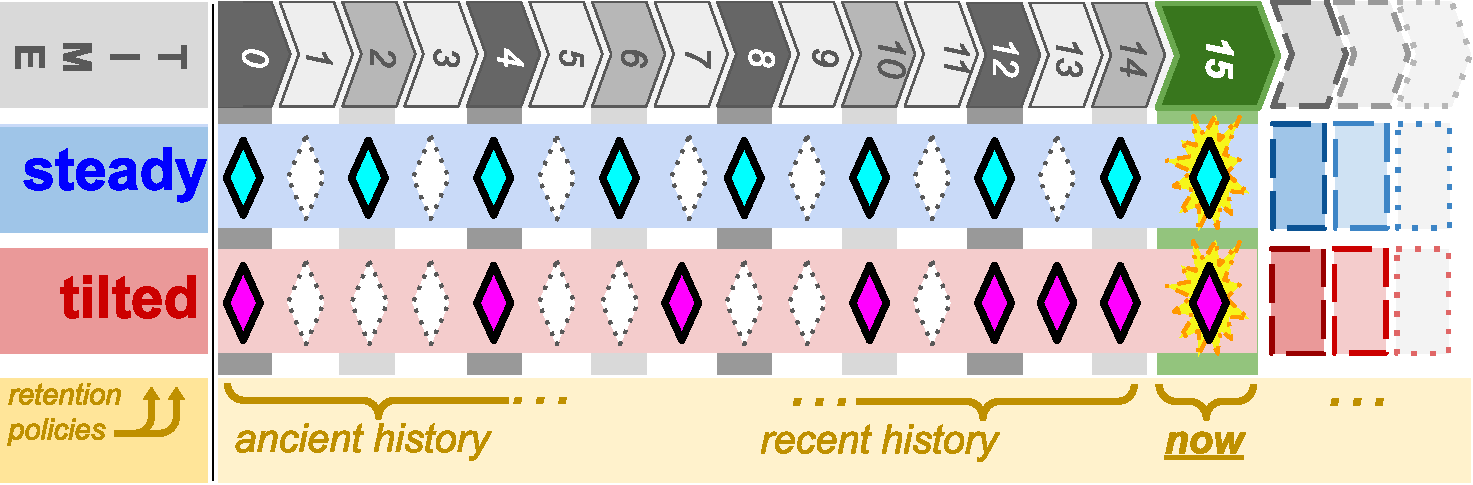
\includegraphics[width=\linewidth]{img/steady-vs-tilted-schematic}
  \caption{%
  \textbf{Steady versus tilted retention policy.}
  Steady policy (top) retains differentia with time points spaced evenly across history.
  Tilted policy (bottom) retains differentia more densely over recent history, giving gap size proportional to time ago.
  Hybrid policy (not shown) allocates half of available space to hold tilted data and half to hold steady.
  }
  \label{fig:steady-vs-tilted-schematic}
\end{figure}


When pruning differentiae, care must be taken to ensure retention of checkpoint generations that maximize coverage across evolutionary history.
In one possible strategy, retained time points would be spread evenly across history.
We term this strategy ``steady'' \citep{han2005stream,zhao2005generalized}.
Such an approach ensures that last common ancestor (LCA) events can be discerned with consistent absolute precision, no matter when they occurred.

Although the steady approach minimizes worst-case imprecision, there is reason to believe it may fail to allocate precision where it would be most useful for discerning phylogenetic history.
In most evolutionary scenarios, there is a general tendency for phylogenetic events concerning extant taxa to have occurred relatively recently \citep{zhaxybayeva2004cladogenesis}.
A strategy accounting for this fact would retain newer time points at higher density than older time points.
We refer to such an approach, where differentiae are retained in a recency-proportional manner, as ``tilted'' \citep{han2005stream,zhao2005generalized}.

Preliminary experiments have indicated that, in some scenarios, annotations using tilted retention can yield higher quality phylogenetic reconstructions than those using steady retention \citep{moreno2022hereditary}.
Experiments here address this question more thoroughly; we assess the relative performance over a variety of evolutionary scenarios, including those expected to maintain greater amounts of ancient history.
In addition, to assess whether benefits of these two approaches can be combined, some experiments consider a third, ``hybrid'' strategy, where annotations are split half-and-half between steady and tilted strategies.

Figure \ref{fig:steady-vs-tilted-schematic} provides a visual comparison of steady and tilted retention strategies.
The steady strategy retains differentia at regular intervals, while the tilted policy retains differentia in proportion to their recency.
Note that these policies must handle continual accrual of new differentia as generations elapse.
At each step, a new differentia is appended, and --- as required --- old differentia are discarded.
Throughout, constraints on time point coverage and annotation size must be respected.
For more detail on algorithmic aspects of this process, see \citet{moreno2024algorithms,moreno2024structured}.

\subsection{Column and Surface-Based Algorithms}
\label{sec:methods-column-vs-surface-algorithms}

Having just described approaches to deciding which differentiae should be stored, we next consider implementation-level approaches to organize and store them in practice.
A suitable annotation data structure for differentiae curation should:
\begin{enumerate}
\item support efficient update operations (to append new differentia and discard old differentiae),
\item be readily serialized (to exchange annotated genomes between processors), and
\item minimize representational overhead (to reduce annotation memory footprint and inter-process message size).
\end{enumerate}

The last point, minimizing representational overhead, is particularly critical given that typical use calls for single-bit and single-byte differentiae.
Requiring 32- or 64-bit pointers or time point values per differentia would cause bookkeeping overhead to greatly outweigh --- and potentially crowd out --- useful lineage history information.
As such, both approaches considered here --- ``column'' and ``surface''-based storage --- pack differentiae in an array format and rely on positional context to identify them.
For such data to be readily legible, retention policies' curated time points must be directly enumerable \textit{a priori} for any arbitrary generation.

The ``column'' approach arranges differentiae in chronological order, with newest differentiae stored last.
This approach suits use of a dynamic array data structure (e.g., Python \texttt{list}/C++ \texttt{std::vector}), as new additions can be accessioned through an append (e.g., ``\texttt{push\_back}'') operation.
Accordingly, the ``column'' approach supports arbitrary growth in curated collection size.
This property allows for retention policies that provide hard guarantees on inference precision.
\footnote{%
Hard fixed or recency-proportional bounds on differentia gap sizes require orders of growth in retention that are linear and logarithmic, respectively \citep{moreno2024algorithms}.
}
One disadvantage to this approach, though, is that discarding old differentia requires an $\mathcal{O}(n)$ shift-down operation on all subsequent elements.

The ``surface'' approach, in contrast, organizes differentiae directly onto a fixed-length buffer \citep{moreno2024structured}.
Rather than appending as a ``\texttt{push\_back}'' on the array, incoming differentiae are assigned an arbitrary buffer position and directly written there in $\mathcal{O}(1)$ time.
One advantage of this approach is that explicit garbage collection operations are unnecessary; new data simply overwrites that to be discarded.
Another advantage is full use of available space --- after the surface buffer is filled, it is guaranteed that stored differentiae fully utilize available capacity.
Owing to discrepancy between projected upper bounds on retained size and actual usage, this guarantee does not hold for column-based tilted retention where maximum size is capped.
However, to the surface approach's disadvantage, dropping a level of abstraction to operate over buffer sites rather than differentia time points results in less fine-grained control over retention and a somewhat looser adherence to idealized retention patterns.
Additionally, by design, growth beyond the surface's fixed buffer size is not supported.
For a more detailed description of motivation for surface-based algorithms, see \citep{moreno2024trackable}.

In sum, the question of column- versus surface-based algorithms can be characterized as a trade-off between efficiency and exactitude.
Indeed, surface-based algorithms provide order-of-magnitude speedups, as well as better compatibility with low-level, resource-constrained programming environments \citep{moreno2024trackable}.
To assess how, if at all, this trade-off impacts reconstruction quality, we include trials using both approaches in empirical annotate-and-reconstruct experiments, described below.
Note that, in these experiments, we consider only fixed-size annotations.
However, we anticipate most hereditary stratigraphy use cases will prefer fixed-size annotation due to practical considerations.


\subsection{Model System}

This section describes the evolution simulations used to generate reference phylogenies for empirical annotate-and-reconstruct experiments.
To support the large, exact-tracked phylogenies needed for this purpose, we used a simple evolution model.
Genomes comprised a single floating-point value, with higher magnitude corresponding to higher fitness.
We used tournament selection with synchronous generations.
Mutation was applied after selection, with a value drawn from a unit Gaussian distribution added to all genomes.
Experiments used asexual reproduction, with no crossover or recombination.
(Extensions of hereditary stratigraphy to sexual lineages are possible \citep{moreno2024methods}, but not explored in this work.)
Evolutionary runs lasted 100,000 generations.

A key consideration in our experiments is assessing reconstruction quality over a breadth of evolutionary scenarios.
To this end, we applied strong, explicit manipulations of evolutionary conditions to explore hereditary stratigraphy methods across diverse regimes of phylogenetic structure.
One focal variable was phylogenetic diversity, the amount of distinct lineage history maintained within an extant population \citep{tucker2017guide}.
For a fixed population size, phylogenetic richness is increased by coexistence of deep phylogenetic branches.
We explored treatments that promote phylogenetic richness via spatial and ecological structure \citep{moreno2024ecology,gomez2019understanding,valiente2007facilitation}.
Spatial structure in experiments was implemented as a simple island population model and ecological structure was implemented as a simple niche model, respectively.

The island model, used to induce spatial structure, distributed individuals evenly across islands, with selection processes taking place in isolation on each island.
Islands were arranged in a one-dimensional closed ring, and 1\% of population members migrated to a neighboring island each generation.

The niche model, used to induce ecological structure, also applies a simple approach.
Organisms were arbitrarily assigned to a niche at simulation startup, with fixed, equally-portioned population slots assigned to each niche.
In the selection procedure, individuals exclusively compete with members of their own niche.
Every generation, individuals swapped niches with probability $3.05 \times 10^{-8}$ (chosen so one niche swap would be expected every 500 generations at the larger population size and 4,000 generations at the smaller).

We also included a drift treatment, where selection was performed in a fully neutral manner.
Drift conditions also enhance phylogenetic richness, but complement other surveyed treatments in operating through a separate mechanism.

Another objective of employing a highly abstracted model to generate reference phylogenies is generality.
Other work with this simple model suggests that effects on phylogenetic structure induced under treatments surveyed here generalize across model systems, albeit to a less accentuated degree \citep{moreno2024ecology}.

In addition to structural aspects of phylogeny composition, we also sought to understand the relationship between population scale and reconstruction quality.
Population sizes of both 4,096 ($2^{12}$) and 65,536 ($2^{16}$) were used in experiments.
We anticipate that many use cases of hereditary stratigraphy will collect and analyze only a subset of extant taxa for tractability of data collection, phylogenetic reconstruction, and phylogenetic analysis.
As such, experiments downsampled generated annotations to 500 taxa.
In experiments using larger population size, we also tested reconstructions over larger samples of 8,000 taxa.

\subsection{Experimental Treatments}

For our main experiments, we defined the following ``regimes'' of evolutionary conditions:
\begin{itemize}
  \item \textit{plain}: tournament size 2 with no niching and no islands,
  \item \textit{mild structure}: tournament size 2 with 2 niches and 4 islands,
  \item \textit{rich structure}: tournament size 2 with 8 niches and 64 islands, and
  \item \textit{drift}: tournament size 1 with no niching and no islands.
\end{itemize}

% for num_generations in 10000 100000; do
% for scope in "export population_size=4096 downsample=500" "export population_size=65536 downsample=500" "export population_size=65536 downsample=8000"; do
% for instrumentation in "export annotation_size_bits=32 differentia_width_bits=1" "export annotation_size_bits=64 differentia_width_bits=1" "export annotation_size_bits=256 differentia_width_bits=1" "export annotation_size_bits=256 differentia_width_bits=8"; do
% for stratum_retention_algo in "surf-steady" "surf-tilted" "surf-hybrid" "col-steady" "col-tilted"; do

% for condition in "export num_islands=1 num_niches=1 tournament_size=2" "export num_islands=1 num_niches=1 tournament_size=1" "export num_islands=4 num_niches=2 tournament_size=2" "export num_islands=64 num_niches=8 tournament_size=2"; do

For each evolutionary regime, we tested four arrangements of annotation capacity and differentia size:
\begin{itemize}
  \item 32-bit array,
  \item 64-bit array,
  \item 256-bit array, and
  \item 32-byte array (256-bit size).
\end{itemize}

Differentia size controls the probability of spurious collision, which is $1/2$ for 1-bit differentia and $1/256$ for 1-byte differentiae, while capacity limitations instead affect the time points where divergence between lineages can be compared.

Treatments also considered \textit{steady-versus-tilted} retention policy and \textit{column-versus-surface} implementation.
Recall that the former determines the overall balance of recent-versus-ancient checkpoints kept and the latter determines the implementation-level particulars of discard sequencing.
Experiments using surface implementation, in addition to steady and tilted approaches, also considered a steady/tilted \textit{hybrid} retention policy.

Across all experiments, each treatment comprised 20 replicates.

\subsection{Agglomerative Phylogeny Reconstruction}

To assess how hereditary stratigraphy would reconstruct ground-truth reference trees, we simulated the inheritance of hereditary stratigraphic annotations along reference phylogenies.
This yielded a set of annotations equivalent to what would be attached to extant population members at the end of a run.
Then, we used the agglomerative tree building implementation provided as \texttt{hstrat.build\_tree} in the \textit{hstrat} Python package \citep{moreno2022hstrat}.
Thus, each reconstruction replicate has a directly corresponding reference tree from an exactly tracked evolution run.

Reconstruction was fast, taking less than a second for the 500-leaf tree with the 256-bit annotation and, in optimized mode, about 5 seconds to build the 8,000-leaf tree.
We then applied a postprocessing step, which took about 20 seconds for the larger tree.

\subsection{Reconstruction Quality Measures}

\begin{figure}
  \centering
  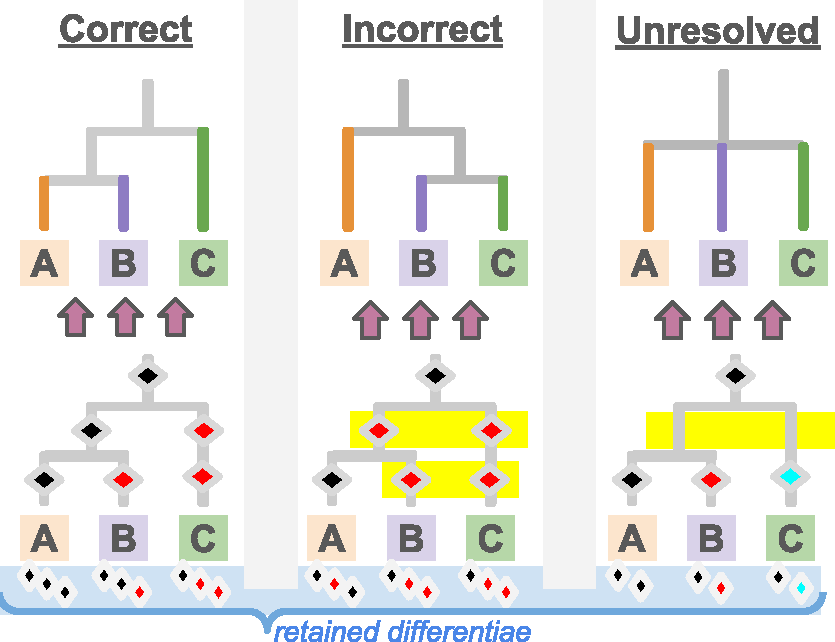
\includegraphics[width=\linewidth]{img/hstrat-failure-modes}
  \caption{%
    \textbf{Differentia structure and reconstruction outcomes.}
    Illustration depicts possible outcomes of reconstruction from hereditary stratigraphy differentia (diamonds) generated and inherited along a two-branch phylogeny (panel bottoms) and resulting reconstruction outcomes (panel tops).
    Diamond placement indicates when differentia were gained and color represents each differentiae's randomly-generated value.
    Diamonds below phylogeny tips summarize inherited hereditary stratigraph record of that taxon.
    \textbf{\textit{Correct reconstruction}} (left panel) occurs when differentia intersperse branching events and differentia value collisions do not occur.
    \textbf{\textit{Incorrect reconstruction}} (center panel) occurs when differentia collisions make unrelated taxa falsely appear related (yellow highlights).
    \textbf{\textit{Unresolved reconstruction}} (i.e., false polytomies; right panel) occurs when differentia do not intersperse branching events but collisions do not occur.
    Note that unresolved reconstructions require differentia size larger than one bit (in order to support $>2$ differentia values), except in the case where more than two differentia records are entirely identical.
  }
  \label{fig:hstrat-failure-modes}
\end{figure}


Assessment of reconstruction quality sought --- in addition to characterizing an overall error measure across hereditary stratigraphy strategies --- to provide diagnostic insight into the nature of reconstruction error produced and the underlying mechanistic reasons it occurs.
Figure \ref{fig:hstrat-failure-modes} depicts two distinct failure modes of hereditary stratigraphy-based reconstruction, which we seek to distinguish.
This example involves three taxa: $A$, $B$, and $C$.
In ground truth, $A$ and $B$ are most closely related and $C$ is an outgroup.
We distinguish three classes of reconstruction outcomes:
\begin{enumerate}
\item \textbf{correct reconstruction}, where retained differentiae suffice to distinguish the $(AB,C)$ branch then the subsequent $(A,B)$ branch;
\item \textbf{incorrect reconstruction}, where spurious differentia collision makes branches appear more closely related than they actually are, e.g., $B$ and $C$ sharing differentiae values by chance, resulting in reconstruction where $B$ and $C$ are inferred as most closely related; and
\item \textbf{unresolved reconstruction}, where differentia necessary to distinguish branching order are not available but subsequent differentia collision does not occur, resulting in artifactual $(A,B,C)$ polytomy.
\end{enumerate}
% An exception is the case where several single-bit differentia records are entirely identical, which results in a polytomy where their leaf nodes derive from a common internal node.

We used triplet distance to assess the overall quality of reconstruction \citep{critchlow1996triples}.
This approach considers all possible three-leaf subsets of a phylogeny, and reports the fraction of triplets with topology mismatching the corresponding triplet in a reference tree.
Triplet distance ranges from 0.0 (between identical trees) to 0.5 (between random trees) to a hypothetical maximum of 1.0.
The triplet distance measure requires that phylogenies are rooted \citep{estabrook1985comparison}.
Conveniently, hereditary stratigraphy produces rooted trees, owing to differentia time points being assigned relative to an explicit generation zero.

To discern error arising from unresolved (as opposed to incorrect) reconstruction, we included a second reconstruction quality measure: inner node loss.
This metric quantifies the difference between the number of inner nodes present in the reference tree versus the reconstruction.
It serves as a precision measure, designed to assess the amount of phylogenetic detail lost due to artifactual polytomies.
Inner node loss ranges from 0.0 (for reconstruction with as many inner nodes as reference) to a maximum of 1.0 (reconstruction is a pathological star phylogeny with only one inner node).
Note that a negative inner node loss might be measured if the reconstruction contains more inner nodes than the reference, owing to erroneous overresolution.
This might occur, for instance, due to the inherent inability of bit-width differentia to represent node degrees higher than bifurcation.
For bit-differentia configurations, this inner node loss measure assumes a very specific interpretation: artifactual polytomies occur exclusively when annotation records share all differentiae in common.
In this case, identical annotations are polytomized as leaves of a single inner node.
% This scenario would likely be AMELIORATED under asynchronous generations on account of leaves being generationally dispersed.

To further discern error from unresolved versus incorrect reconstruction, we occasionally distinguish an alternate ``lax'' triplet distance from the ``strict'' triplet distance measure described above.
Lax triplet distance differs from strict triplet distance in that it does not penalize triplets that mismatch on account of polytomy.
This measure is useful in isolating incorrect reconstruction from unresolved reconstruction.
However, care should be taken in interpreting lax triplet distance, as the pathological ``star'' tree case where all leaves descend directly from the root in one large polytomy would measure zero reconstruction error under the lax triplet distance measure.
As such, where used, strict triplet distance is also reported.
Where not specified, triplet distance refers to the strict measure.

% 
\begin{figure*}
  \centering

\begin{subfigure}[b]{\textwidth}
\centering
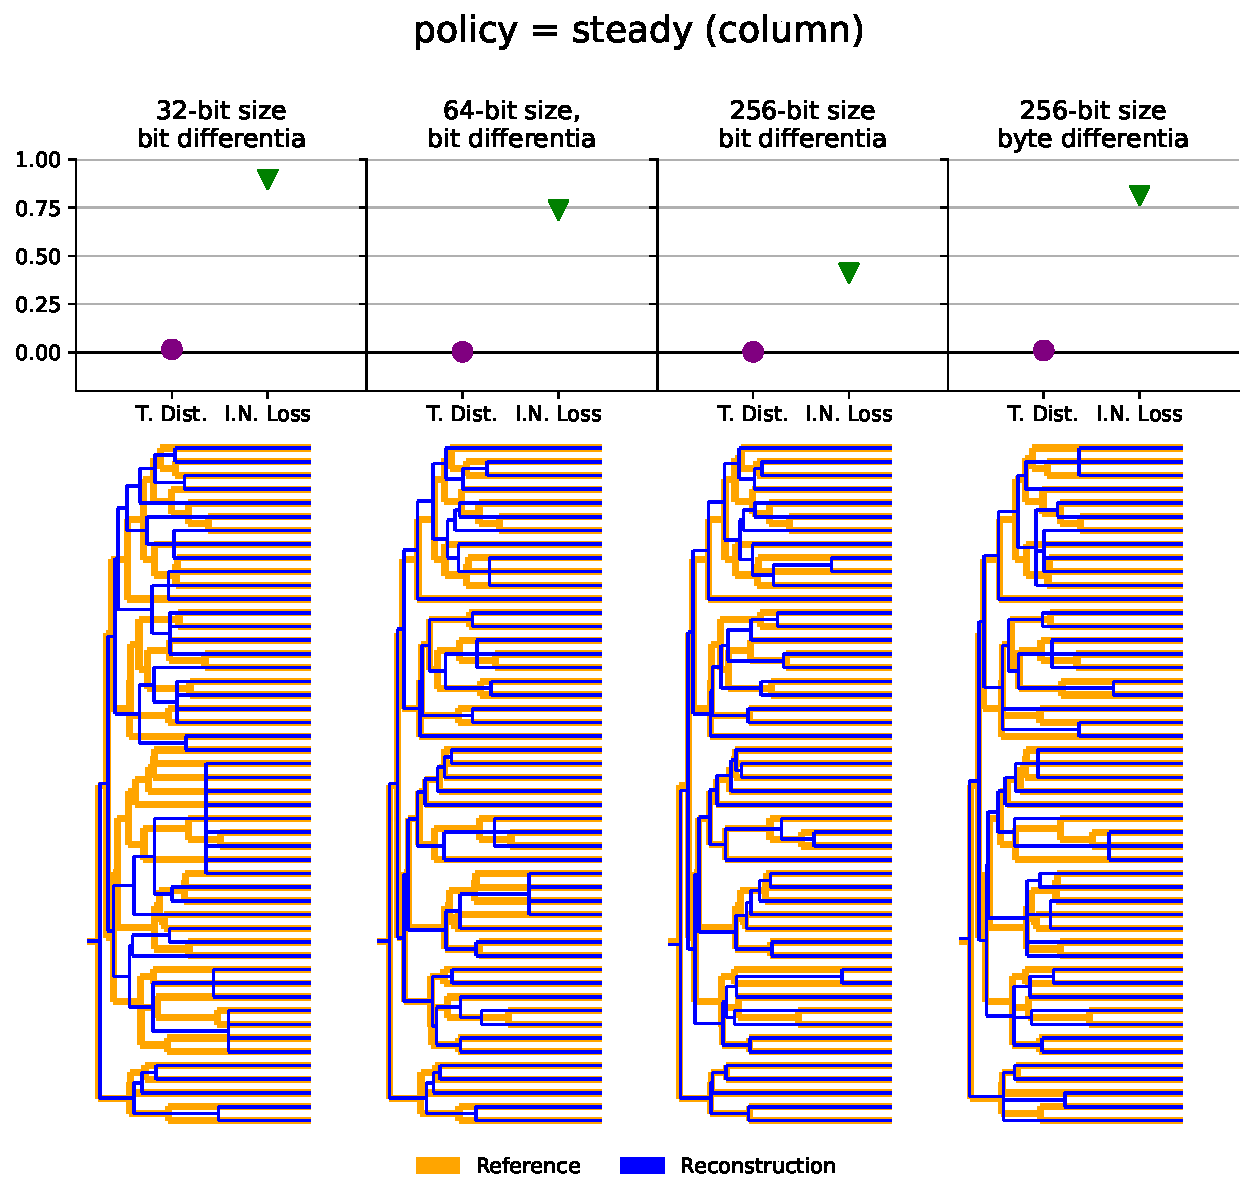
\includegraphics[width=0.5\textwidth]{binder/binder/outplots/a=examplepanel+policy=col-steady+regime=drift+ext=}%
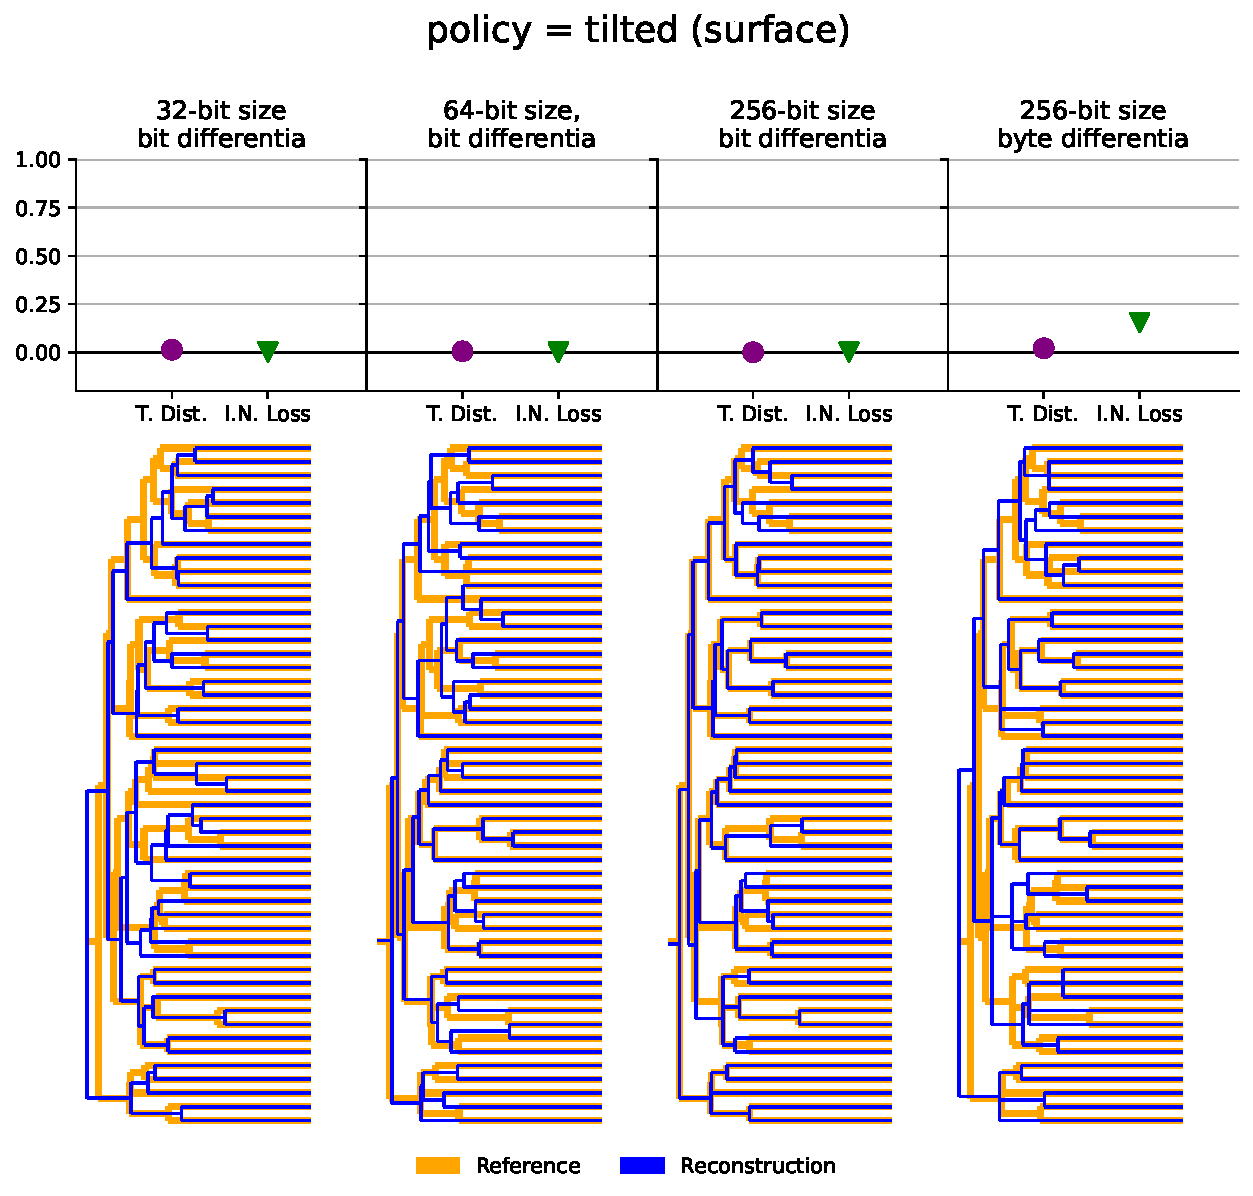
\includegraphics[width=0.5\textwidth]{binder/binder/outplots/a=examplepanel+policy=surf-tilted+regime=drift+ext=}
\caption{drift regime --- high phylogenetic richness}
\label{fig:examplepanel-drift}
\end{subfigure}

\begin{subfigure}[b]{\textwidth}
\centering
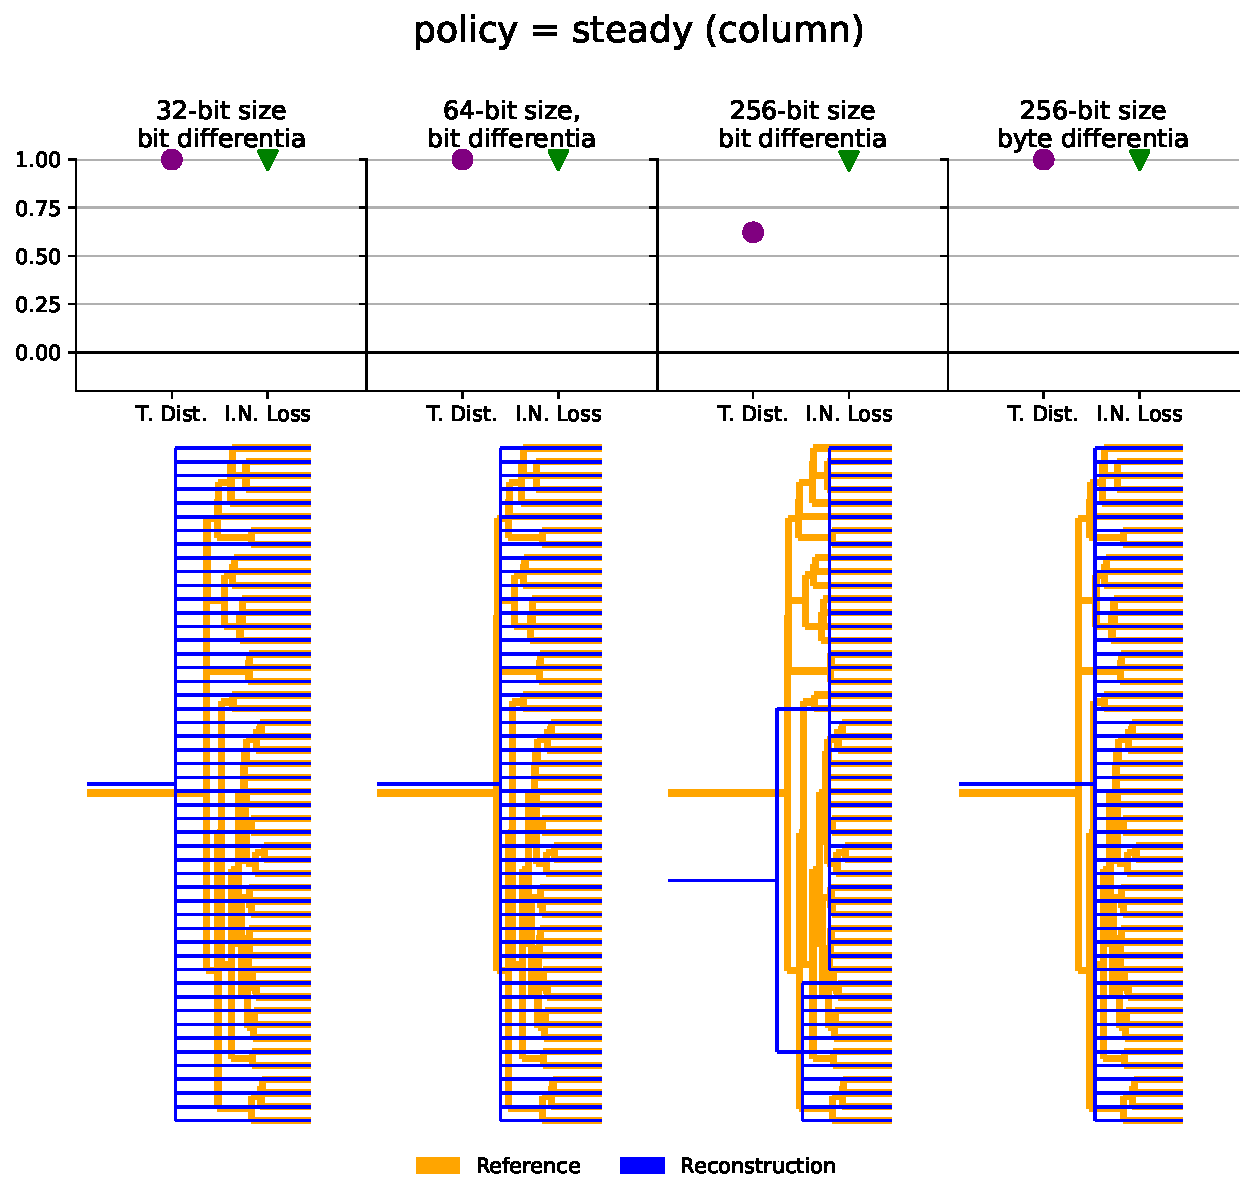
\includegraphics[width=0.5\textwidth]{binder/binder/outplots/a=examplepanel+policy=col-steady+regime=plain+ext=}%
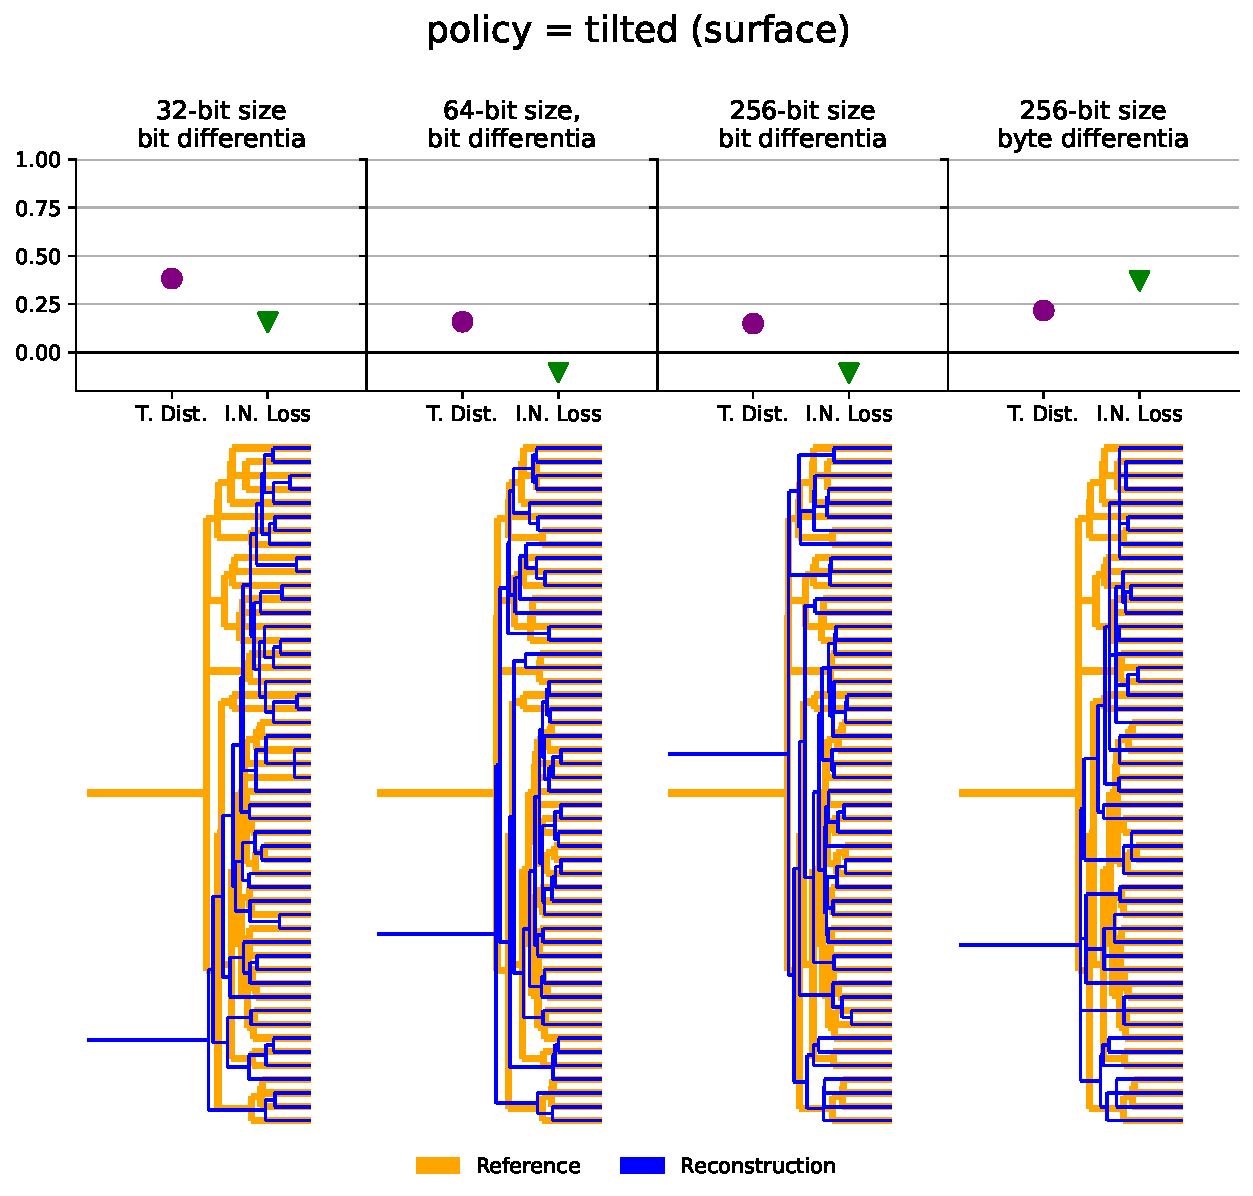
\includegraphics[width=0.5\textwidth]{binder/binder/outplots/a=examplepanel+policy=surf-tilted+regime=plain+ext=}
\caption{plain regime --- low phylogenetic richness}
\label{fig:examplepanel-plain}
\end{subfigure}

  \caption{%
  \textbf{Reconstruction vs. Reference Examples.}
  Comparison of reconstruction to reference tree for steady and tilted policies under drift (\ref{fig:examplepanel-drift}) and plain (\ref{fig:examplepanel-plain}) evolutionary regimes.
  Panel tops show reconstruction quality metrics and panel bottoms overlay reconstruction (blue) on reference tree (orange). 
  Phylogeny time axes are log scale.
  Note that overlay layout is naive, so can underrepresent agreement between trees; however, comparison is informative to general differences in tree structure.
  }
  \label{fig:examplepanel}

\end{figure*}


% Figure \ref{fig:examplepanel} shows example reference phylogenies, corresponding reconstructions, and quality metrics in practice.
% The top panel shows trials from the drift treatment, which exhibits high phylogenetic richness, and the bottom panel shows trials from the plain treatment, which exhibits low phylogenetic richness.
% (Note that, for legibility, time axes of phylogenies are log-scaled, which somewhat reduces the apparent visual distinction of high-versus-low phylogenetic richness.)
% Each panel compares reconstruction results under steady (left) and recency-proportional (right) instrumentation.
% Particularly high incidence of node loss (green triangle) can be seen under steady retention.
% Correspondingly, many large polytomies can be seen in the example steady-retention reconstructions (blue overlaid dendrogram) compared to the corresponding reference phylogeny (orange underlaid dendrogram).
% Under the plain treatment, steady retention leads to particularly high (almost complete) inner node loss, and --- correspondingly --- triplet distance similarity (purple dots) is very poor.
% Despite high inner node loss under the drift treatment, triplet distance remains low under steady retention.
% Across example cases shown, tilted retention enjoys triplet distance and inner node loss comparable to or better than steady retention.
% The main discussion will return to explore this question of steady-versus-tilted retention in greater rigor and depth.

\subsection{Statistical Methods}

Comparisons of reconstruction quality considered both statistical significance (the likelihood an observed difference between treatments might have occurred by chance) and effect size (the magnitude of distinction between treatments relative to outcome variabilities).
We used nonparametric methods for both analyses.
By assessing effect sign, size, and significance across treatment conditions, we described the extent and consistency with which one instrumentation approach outperformed others.

We used Cliff's delta to report effect size.
This statistic describes the proportion of distributional non-overlap between two distributions, ranging from 1 (or -1) if two distributions share no overlap to 0 if they overlap entirely \citep{cliff1993dominance}.
When reporting effect size, we use conventional thresholds of 0.147, 0.33, and 0.474 to distinguish between negligible, small, medium, and large effect sizes \citep{hess2004robust}.
Note that the Cliff's delta statistic tops/bottoms out entirely once two distributions become completely separable.
Where appropriate, we additionally report effects directly in terms of the underlying quality metrics.

We pair effect-size analysis with Mann-Whitney U testing in order to assess evidence that significant differences exist between reconstruction quality under different conditions \citep{mann1947on}.
As our goal was to screen for possible effects, rather than establish the veracity of any one effect, we did not correct for multiple comparisons in assessing statistical significance.
Because incorrectly identifying a lack of difference between conditions would be more harmful than incorrectly identifying the presence of a difference, this approach is conservative in maintaining the sensitivity of our assays.
Where we do detect a significant effect, we additionally report results after applying Bonferroni correction.

When determining the best- and worst-performing among three or more hereditary stratigraphy approaches, we use a nonparametric skimming procedure provided by the \textit{pecking} Python library \citep{moreno2024pecking}.
The procedure first applies a Kruskal-Wallis H-test to determine if there is evidence for significant variation among the sample groups.
If this test fails, then no best- or worst-performing group or groups are identified.
If a significant difference is found, observation ranks are calculated and sample groups are sorted in order of mean rank.
To discern the lowest-ranked group(s), successive Mann-Whitney U-tests are performed between the lowest-rank group and successively higher-ranked groups, adjusting the significance level $\alpha$ for multiple comparisons according to a sequential Holm-Bonferroni procedure.
The overall lowest-ranked group and subsequent groups tested before encountering the first significantly differing group are taken as the best-performing (given that the metric in question is an error measure).
This approach, therefore, identifies the set of lowest-ranked groups that are statistically indistinguishable amongst themselves.
A similar procedure is used to identify a set of highest-ranked groups.
